\section{Amostragem - principais erros}

\begin{frame}	
	\begin{block}{Amostras viesadas}	
		\begin{itemize}
			\item Precisamos de informação precisa e sem viés para tomarmos boas decisões.
			\item Se você ``cria conhecimento' ou ``toma decisões'' usando informação viesada você não está sendo \# datadriven
			\item A probabilidade de tomar decisões ruins aumenta... e decisões ruins costumam ser caras...
		\end{itemize}		
	\end{block}
\end{frame}

\begin{frame}	
	\begin{block}{processo de KDD}	
		\begin{figure}[!htb]
			\centering	  				
			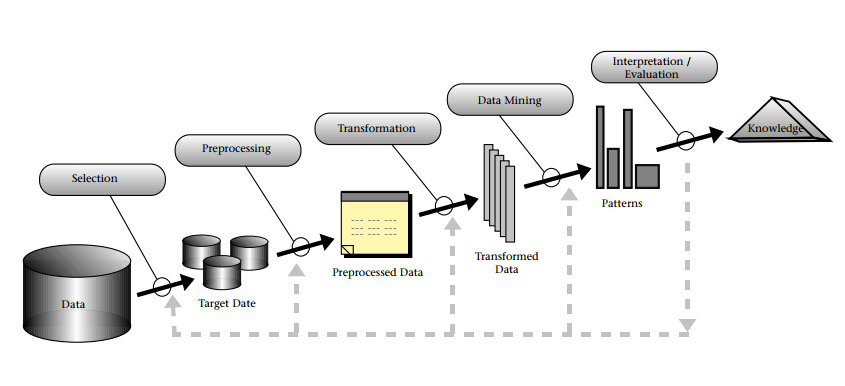
\includegraphics[height=5cm, width = 12cm]{./pic/kddprocess.jpg}
			\caption{Processo de KDD}
			\label{fig_kdd_process}
		\end{figure}
		\begin{itemize}
			\item Se você cometer um erro durante a etapa de: ``seleção'' os passos seguintes e suas conclusões estarão erradas.
		\end{itemize}
	\end{block}
\end{frame}

\begin{frame}	
	\begin{block}{Amostragem 101}	
		\begin{figure}[!htb]
			\centering	  				
			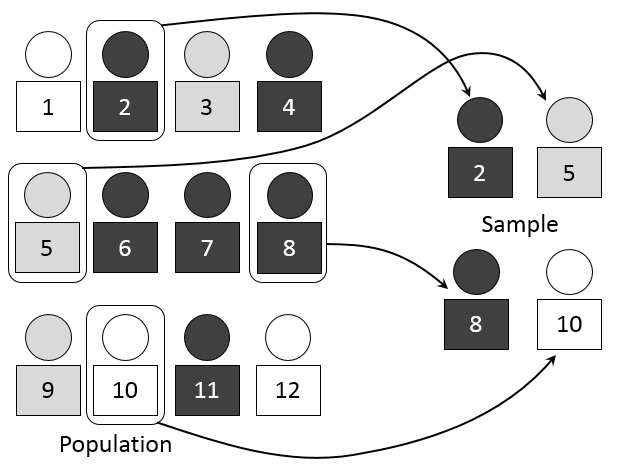
\includegraphics[height=5cm, width = 12cm]{./pic/sampling.png}
			\caption{Overview de amostragem}
			\label{fig_sampling}
		\end{figure}
		\begin{itemize} 
			\item O subconjunto (amostra) de elementos deve ser representativa da população.
		\end{itemize}
	\end{block}
\end{frame}

\begin{frame}	
	\begin{block}{Bias de auto seleção}	
		\begin{itemize} 
			\item Suponha um estudo estatístico sobre detalhes íntimos da sexualidade de estudantes em universidades. Algumas pesssoas provavelmente vão mentir.
			\item Uma pesquisa online sobre quem gosta de usar computador.
			\item Em ambos as pessoas selecionadas vão terão seus comportamentos diferentes da população geral.
		\end{itemize}
	\end{block}
\end{frame}


\begin{frame}	
	\begin{block}{Undercoverage Bias}	
		\begin{itemize} 
			\item Digest em 1936 fez uma pesquisa eleitoral que previa vitória larga do candidato Lando em relação ao candidato Roosevelt. Roosevelt ganhou com uma margem larga, a pesquisa era feita por telefone, na época pessoas pobres (maioria da população que era a favor de Roosevelt) não tinha telefone. Essa foi uma das causas do erro estatístico.
		\end{itemize}
	\end{block}
\end{frame}

\begin{frame}	
	\begin{block}{Survivorship Bias}	
		\begin{itemize} 
			\item Ocorre quando as observações estudadas no fim da investigação são não aleatórias em comparação as presentes no começo da observação.		
		\end{itemize}
	\end{block}
\end{frame}


\begin{frame}	
	\begin{block}{Survivorship Bias}	
		\begin{itemize} 
			\item Exemplo da segunda guerra mundial (tiros em avião)
		\end{itemize}
	\end{block}
\end{frame}

